%%%%%%%%%%%%%%%%%%%%%%%%%%%%%%%%%%%%%%%%%%%%%%%%%%%%%%%%%%%%%%%%%%%%%%%%%%%%%%%%%%%%%%%
%%%%%%%%%%%%%%%%%%%%%%%%%%%%%%%%%%%%%%%%%%%%%%%%%%%%%%%%%%%%%%%%%%%%%%%%%%%%%%%%%%%%%%%
% 
% This top part of the document is called the 'preamble'.  Modify it with caution!
%
% The real document starts below where it says 'The main document starts here'.

\documentclass[12pt]{article}

\usepackage{amssymb,amsmath,amsthm}
\usepackage[top=1in, bottom=1in, left=1.25in, right=1.25in]{geometry}
\usepackage{fancyhdr}
\usepackage{graphicx}
\usepackage{enumerate}
\usepackage{verbatim}
\usepackage{listings}
\usepackage{float}

% Comment the following line to use TeX's default font of Computer Modern.
\usepackage{times,txfonts}

\newtheoremstyle{homework}% name of the style to be used
  {18pt}% measure of space to leave above the theorem. E.g.: 3pt
  {12pt}% measure of space to leave below the theorem. E.g.: 3pt
  {}% name of font to use in the body of the theorem
  {}% measure of space to indent
  {\bfseries}% name of head font
  {:}% punctuation between head and body
  {2ex}% space after theorem head; " " = normal interword space
  {}% Manually specify head
\theoremstyle{homework} 

% Set up an Exercise environment and a Solution label.
\newtheorem*{exercisecore}{\@currentlabel}
\newenvironment{exercise}[1]
{\def\@currentlabel{#1}\exercisecore}
{\endexercisecore}

\newcommand{\localhead}[1]{\par\smallskip\noindent\textbf{#1}\nobreak\\}%
\newcommand\solution{\localhead{Solution:}}



% \newcommand{includematlab}[1]{\verbatiminput{#1}}

%%%%%%%%%%%%%%%%%%%%%%%%%%%%%%%%%%%%%%%%%%%%%%%%%%%%%%%%%%%%%%%%%%%%%%%%
%
% Stuff for getting the name/document date/title across the header
\makeatletter
\RequirePackage{fancyhdr}
\pagestyle{fancy}
\fancyfoot[C]{\ifnum \value{page} > 1\relax\thepage\fi}
\fancyhead[L]{\ifx\@doclabel\@empty\else\@doclabel\fi}
\fancyhead[C]{\ifx\@docdate\@empty\else\@docdate\fi}
\fancyhead[R]{\ifx\@docauthor\@empty\else\@docauthor\fi}
\headheight 15pt

\def\doclabel#1{\gdef\@doclabel{#1}}
\doclabel{Use {\tt\textbackslash doclabel\{MY LABEL\}}.}
\def\docdate#1{\gdef\@docdate{#1}}
\docdate{Use {\tt\textbackslash docdate\{MY DATE\}}.}
\def\docauthor#1{\gdef\@docauthor{#1}}
\docauthor{Use {\tt\textbackslash docauthor\{MY NAME\}}.}
\makeatother

%% General formatting parameters
\parindent 0pt
\parskip 12pt plus 1pt

\def\vx{\mathbf x}
\def\vb{\mathbf b}

% Shortcuts for blackboard bold number sets (reals, integers, etc.)
\newcommand{\Reals}{\ensuremath{\mathbb R}}
\newcommand{\Nats}{\ensuremath{\mathbb N}}
\newcommand{\Ints}{\ensuremath{\mathbb Z}}
\newcommand{\Rats}{\ensuremath{\mathbb Q}}
\newcommand{\Cplx}{\ensuremath{\mathbb C}}
%% Some equivalents that some people may prefer.
\let\RR\Reals
\let\NN\Nats
\let\II\Ints
\let\CC\Cplx

%%%%%%%%%%%%%%%%%%%%%%%%%%%%%%%%%%%%%%%%%%%%%%%%%%%%%%%%%%%%%%%%%%%%%%%%%%%%%%%%%%%%%%%
%%%%%%%%%%%%%%%%%%%%%%%%%%%%%%%%%%%%%%%%%%%%%%%%%%%%%%%%%%%%%%%%%%%%%%%%%%%%%%%%%%%%%%%
% 
% The main document start here.

% The following commands set up the material that appears in the header.

%%%%%%%%%%%%%%%%%%%%%%%%%%%%%%%%%%%%%%%%%%%%%%%%%%%%%%%%%%%%%%%%%%%%%%%%%%
\doclabel{Math 426: Homework 13}
\docauthor{Stefano Fochesatto}
\docdate{\today}

\begin{document}


\begin{exercise}{Problem 10.5} The Chebyshev polynomials $T_j(x)  = cos(j arccos(x))$, $j = 0,1,\dots,$ are orthogonal with respect to the
    weight function $(1 - x^2)^{-1/2}$ on $[-1,1];$ that is $\int_{-1}^{1} T_j(x)T_k(x)(1 - x^2)^{-1/2} dx = 0$ if $j \neq k$. Use the Gram-Schmidt
    process applied to the linearly independent set $\{1, x, x^2\}$ to construct the first three orthonormal polynomials for this weight function
    and show that they are indeed scalar multiples of $T_0, T_1, T_2$\\

    \solution First let $w =(1 - x^2)^{-1/2}$. Then using the Gram-Schmidt process to construct $q_0, q_1, q_2$ $w$-orthogonal polynomials on the set $\{1, x, x^2\}$.
    Let $q_0 = 1$, then 
    \begin{align*}
        q_1(x) &= x - \dfrac{<x,1>_w}{<1,1>_w} 1\\
        &= x - \dfrac{\int_{-1}^{1} x(1 - x^2)^{-1/2}dx}{\int_{-1}^{1} x(1 - x^2)^{-1/2}dx}\\
        &= x - \dfrac{0}{\pi} = x.
    \end{align*}
    Solving for $q_2$ that is orthogonal to $q_0, q_1$,
    \begin{align*}
        q_2(x) &= x^2 - \dfrac{<x^2,1>_w}{<1,1>_w} 1 - \dfrac{<x^2,x>_w}{<x,x>_w} x,\\
        &= x^2 - \dfrac{\int_{-1}^{1} x^2(1 - x^2)^{-1/2}dx}{\int_{-1}^{1} x(1 - x^2)^{-1/2}dx} - \dfrac{\int_{-1}^{1} x^3(1 - x^2)^{-1/2}dx}{\int_{-1}^{1} x^2(1 - x^2)^{-1/2}dx}x,\\
        &= x^2 - \dfrac{(\pi/2)}{\pi} - \dfrac{0}{\pi}x,\\
        &= x^2 - \dfrac{(\pi/2)}{\pi}.
    \end{align*}
    Finally normalizing each polynomial we get the following,
    \begin{equation*}
        \hat{q}_0 = \dfrac{1}{<1,1>} = \dfrac{1}{\sqrt(\int_{-1}^{1}1 dx)} = \dfrac{1}{\sqrt{2}},
    \end{equation*}
    
    \begin{equation*}
        \hat{q}_1 = \dfrac{x}{<x,x>} = \dfrac{1}{\sqrt(\int_{-1}^{1} x^2 dx)} = \dfrac{\sqrt{3}x}{\sqrt{2}},
    \end{equation*}
    
    \begin{equation*}
            \hat{q}_2 = \dfrac{x^2 - \dfrac{(\pi/2)}{\pi}}{<q_2,q_2>}= \dfrac{x^2 - \dfrac{(\pi/2)}{\pi}}{\sqrt(\int_{-1}^{1} (x^2 - \dfrac{(\pi/2)}{\pi})^2 dx)} = \dfrac{\sqrt{30}(x^2 - \dfrac{(\pi/2)}{\pi})}{\sqrt{7}}.
    \end{equation*}
    Calculating the first three Chebyshev Polynomials.
    \begin{equation*}
        T_0 = cos(0 arccos(x)) = 1,
    \end{equation*}
    \begin{equation*}
        T_1 = cos(arccos(x)) = x.
    \end{equation*}
    Using the double angle identity, and pythagorean theorem,
    \begin{align*}
        T_2 &= cos(2 arccos(x)),\\
        &= cos^2(arccos(x))  - sin^2(arccos(x)),\\
        &= x^2 - (1 - x^2),\\
        &= 2x^2 - 1.
    \end{align*}
    Now we can see that we get the following scalar multiples,
    \begin{align*}
        T_0 &= \dfrac{1}{\sqrt{2}}\hat{q}_0,\\
        T_1 &= \dfrac{\sqrt{2}}{\sqrt{2}}\hat{q}_1,\\
        T_2 &= \dfrac{\sqrt{30}}{2\sqrt{7}}\hat{q}_2.
    \end{align*} 
\end{exercise}
\vspace{.5in}









\begin{exercise}{Problem 10.7} Write a MATLAB code to approximate,
    \begin{equation*}
        \int_0^1 cos(x^2) dx
    \end{equation*}
    Using composite trapezoid rule and one to approximate the integral using the composite Simpson's rule, with equally-spaced, nodes.
    The number of intervals $n = 1/h$ should be and input to each code.\\
    Do a convergence study to verify the second-order accuracy of the composite trapezoid rule and the fourth-order accuracy of the 
    composite Simpson's Rule;\\

    \solution
    \textbf{Function:}
    \begin{center}
    \lstinputlisting{Trap.m}
    \end{center}
    
    \textbf{Function:}
    \begin{center}
    \lstinputlisting{Simpsons.m}
    \end{center}

    \textbf{Console:}
    \begin{center}
    \lstinputlisting{convergence_trap.txt}
    \end{center}
    
    \begin{center}
    \begin{tabular}{llll}
        $1/h$ & $T_h$ & $E_h$ & $E_h/h^2$ \\ 
        \hline 
        1 & 0.77015 & 0.13437 & 0.13437 \\ 
        10 & 0.90312 & 0.0014025 & 0.14025 \\ 
        100 & 0.90451 & 1.4025e-05 & 0.14025 \\ 
        1000 & 0.90452 & 1.4025e-07 & 0.14025 \\ 
        10000 & 0.90452 & 1.4025e-09 & 0.14025 \\ 
        100000 & 0.90452 & 1.4039e-11 & 0.14039 \\ 
        \hline 
    \end{tabular}
    \end{center}

    \textbf{Console:}
    \begin{center}
    \lstinputlisting{convergence_simp.txt}
    \end{center}

    \begin{center}
        \begin{tabular}{llll}
            $1/h$ & $T_h$ & $E_h$ & $E_h/h^4$ \\ 
            \hline 
            2 & 0.9045 & 2.2972e-05 & 0.00036755 \\ 
            4 & 0.90452 & 7.8693e-08 & 2.0145e-05 \\ 
            8 & 0.90452 & 1.4667e-08 & 6.0077e-05 \\ 
            16 & 0.90452 & 1.2157e-09 & 7.967e-05 \\ 
            32 & 0.90452 & 8.0618e-11 & 8.4534e-05 \\ 
            64 & 0.90452 & 5.1057e-12 & 8.5659e-05 \\ 
            128 & 0.90452 & 3.1475e-13 & 8.449e-05 \\ 
            256 & 0.90452 & 1.41e-14 & 6.0558e-05 \\ 
            \hline 
            \end{tabular}
        \end{center}
    






\end{exercise}
\vspace{.5in}









\begin{exercise}{Supplimental 1} Continuing with the theme that some sample points are better than others, recall that polynomial interpolation with high-order polynomials is prone to making large oscillation errors, but that this can be minimized
using Chebyshev polynomials, which are the Lagrange polynomials associated
with the sample points 
\[
x_j= \cos(\pi+(\pi j/n)),\qquad j=0,\ldots,n
\]
on the interval $[-1,1]$.
Clenshaw-Curtis integration is integration using polynomial interpolation at
these sample points.

Use the MATLAB \texttt{polyfit} function to perform polynomial
interpolation at these sample points for $n=4,6,10$ and then
use the resulting polynomials to approximate
\[
\int_{-1}^1 x\sin(x)\;dx.
\]
Compare your approximations to the exact answer (which you should
compute by hand).  Integration by parts!\\

\solution Computing the value of the integral by hand using integration by parts,
\begin{align*}
    \int_{-1}^1 x\sin(x)\;dx &=  -x\cos(x)|_{-1}^1 -\int_{-1}^1-\cos(x)\;dx,\\
     &=  -x\cos(x) - (-\sin(x))|_{-1}^1,\\
     &=  -x\cos(x) + \sin(x)|_{-1}^1,\\
     &= -2\cos(1)+2\sin(1).
\end{align*}
Using the following MATLAB function to approximate the integral, with a Chebyshev polynomial interpolant
of degree 4,6, and 10.\\
\textbf{Function:}
\begin{center}
\lstinputlisting{cheby_inter.m}
\end{center}

\textbf{Console:}
\begin{center}
\lstinputlisting{cheby_inter.txt}
\end{center}


\end{exercise}
\vspace{.5in}




\begin{exercise}{Supplimental 2} Recall that 5 point Gauss-Legendre integration
uses sample points
$[-\beta,-\alpha,0,\alpha,\beta]$ where
\[
\begin{aligned}
\alpha &= \frac{1}{3}\sqrt{5-2\sqrt{\frac{10}{7}}}\\
\beta &= \frac{1}{3}\sqrt{5+2\sqrt{\frac{10}{7}}}.
\end{aligned}
\]
Write a code that performs composite Gauss-Legendre integration
with these sample points.  Your code should have the signature
\begin{verbatim}
function q=glquad(f,a,b,N)
...
end
\end{verbatim}
were $f$ is the function to integrate, $a$ and $b$ are the endpoints
of integration, and $N$ is the number of subintervals. Your code
should perform Gauss-Legendre integration on each subinterval and add them up.
Then apply your function to compute
\[
\int_{-1}^1 x\sin(x)\;dx
\]
using $N=1,2,4,10$.  Compare the results of Gauss-Legendre integration
to the results you saw using Clenshaw-Curtis integration.\\

\solution

\textbf{Function:}
\begin{center}
\lstinputlisting{glquad.m}
\end{center}

\textbf{Console:}
\begin{center}
\lstinputlisting{glquad_comp.txt}
\end{center}
Clearly we are seeing faster convergence using the Gauss-Legendre integration. Doing an approximation for 
$n = 1,2,\dots,10$ and plotting the absolute errors against our value of $n$ we can see that Gauss-Legendre integration
reaches higher precision at lower values of $n$.\\

\begin{figure}[h]
    \caption{Integration Technique Comparison}
    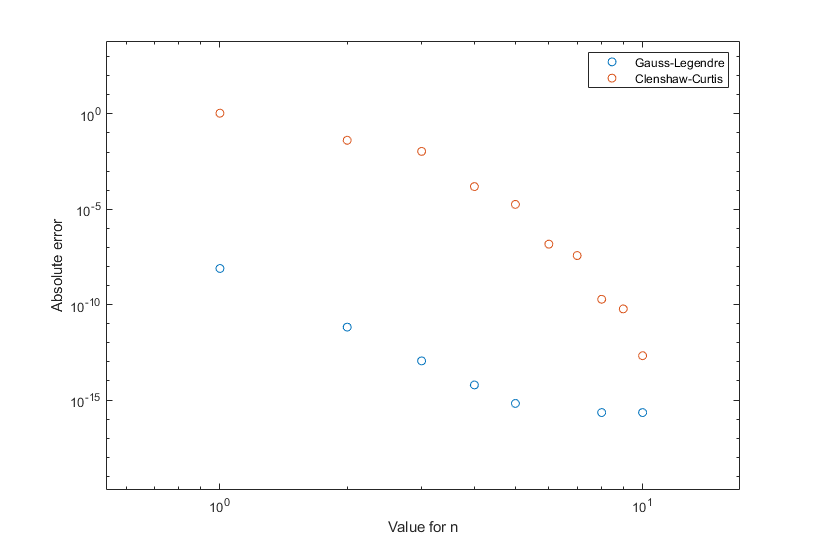
\includegraphics[width = \textwidth]{error analysis.png}  
    \centering
  \end{figure}
\end{exercise}
\vspace{.5in}


\begin{exercise}{Problem 9.1} Use MATLAB to evaluate the second-order-accurate approximation
    to $f''(x)$ for $f(x) = sin(x)$ and $x = \pi/6$. Try $h = 10^{-1}, 10^{-2}, \dots, 10^{-16}$
    and make a table of values of $h$, the computed finite difference quotient, and the error. Explain your results.\\
\solution 

\textbf{Function:}
\begin{center}
\lstinputlisting{diff_2.m}
\end{center}

\textbf{Console:}
\begin{center}
\lstinputlisting{diff_2.txt}
\end{center}

\begin{center}
\begin{tabular}{lll}
    $h$ & $f''(pi/6)$ & $E_{d2}$ \\ 
    \hline 
    0.1 & -0.49958 & 0.00041653 \\ 
    0.01 & -0.5 & 4.1667e-06 \\ 
    0.001 & -0.5 & 4.1674e-08 \\ 
    0.0001 & -0.5 & 3.0387e-09 \\ 
    1e-05 & -0.5 & 5.9648e-07 \\ 
    1e-06 & -0.49993 & 6.6572e-05 \\ 
    1e-07 & -0.49405 & 0.0059508 \\ 
    1e-08 & -1.1102 & 0.61022 \\ 
    1e-09 & 55.5112 & 56.0112 \\ 
    1e-10 & 0 & 0.5 \\ 
    1e-11 & 0 & 0.5 \\ 
    1e-12 & 0 & 0.5 \\ 
    1e-13 & 5551115123.1258 & 5551115123.6258 \\ 
    1e-14 & -555111512312.5782 & 555111512312.0782 \\ 
    1e-15 & 0 & 0.5 \\ 
    1e-16 & -5551115123125783 & 5551115123125782 \\ 
    \hline 
    \end{tabular}
\end{center}
From our error analysis we can see that our best approximation comes when $h = 10^{-4}$. Looking at the Taylor's
Theorem formula for $f''(x)$ in Example 9.1.2 we get that,
\begin{equation*}
    f''(x) = \dfrac{f(x+h) - 2f(h) + f(x - h)}{h^2} - \dfrac{h^2}{12}f''''(v)
\end{equation*}
We see that the error will be $O(h^2)$. Following a similar analysis as example 9.1.1 we see that the minimum computed difference
quotient is on the order of $O(\epsilon/h^2)$. Solving for $h$ we get that $h = \epsilon^{\frac{1}{4}}\approx 10^{-4}$.  
\end{exercise}
\vspace{.5in}



\begin{exercise}{Problem 9.5} Using Taylor series, derive the error term for the approximation,\\

    \solution 

    \begin{equation*}
        f'(x) \approx \dfrac{1}{2h}[-3f(x) + 4f(x+h) - f(x + 2h)].
    \end{equation*}
    Applying the Taylor series formula to each function, we ge the following system,
    \begin{equation*}
        -3f(x) = -3f(x).
    \end{equation*}
    \begin{equation*}
        4f(x + h) = 4f(x) + 4f'(x)h + \dfrac{4f'(x)h^2}{2!} + \dfrac{4f'(x)h^3}{3!} + O(h^4).
    \end{equation*}
    \begin{equation*}
        -f(x + 2h) = -f(x)  - 2f'(x)h  - \dfrac{4f'(x)h^2}{2!} - \dfrac{8f'(x)h^3}{3!} + O(h^4).
    \end{equation*}
    Summing over the equation we get that,
    \begin{equation*}
        [-3f(x) + 4f(x+h) - f(x + 2h)] = 2f'(x)h - \dfrac{4f'(x)h^3}{3!} + O(h^4).
    \end{equation*}
    Finally we divide the whole equation by $2h$ to get,
    \begin{equation*}
        \dfrac{[-3f(x) + 4f(x+h) - f(x + 2h)]}{2h} = f'(x) - \dfrac{2f'(x)h^2}{3!} + O(h^3).
    \end{equation*}
    Thus the error term is,
    \begin{equation*}
        error = -\dfrac{2f'(x)h^2}{3!} + O(h^3).
    \end{equation*}
\end{exercise}







\end{document}